
\section{Implementation}


\subsection{Operation}
Text editing can be realized with only two operations. 
 - Insert
 - Delete
 - Split

All operations have some equivalent properties. They must provide a function called \texttt{inverse()} that returns the inverse operation, a . 

They are represented by the Operation Interface.
 
\subsubsection{Operation Hierarchy}
\begin{figure}[H]
\centering
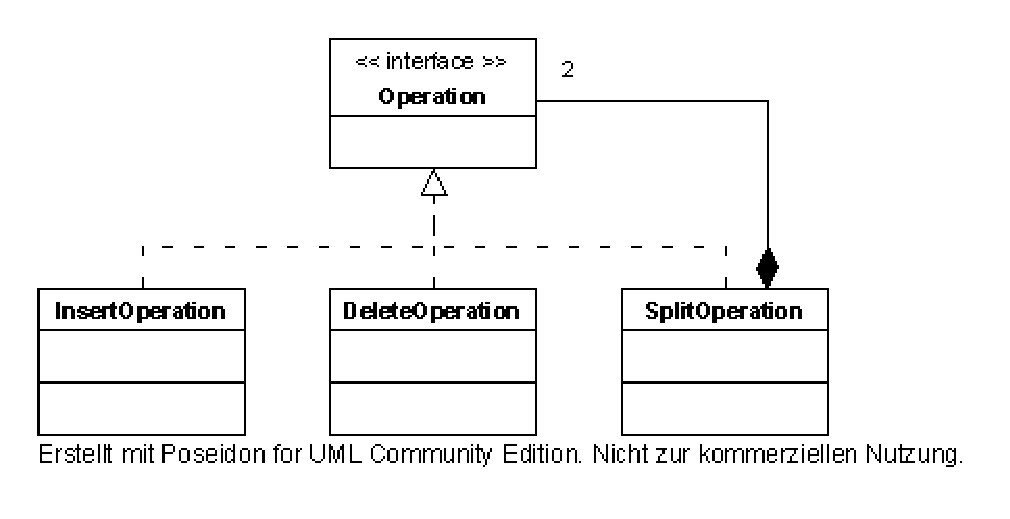
\includegraphics[height=4cm,width=8cm]{../../images/algo-impl/operation.eps}
\caption{Operation Hierarchy}
\end{figure}

\subsubsection{InsertOperation}


\subsubsection{DeleteOperation}
\subsubsection{SplitOperation}
  - no operation
  - wrapper to handle special cases -> \ref{Delete_Insert}


\subsection{Request}

\newpage
\subsection{GOTO Transformation Functions}

\subsubsection{Overview}
The GOTO (generic operation transformation optimized) transformation functions are designed to work with strings. The advantage is that less transformations are needed when a string has been inserted into a text. To understand the exigence of transformation functions see \emph{Evaluation Algorithms}.

The inclusion transformation functions are used to check the influence of a given operation B to another operation A. If so, the operation A will be transformed into operation A'. To transform an operation means to adapt position and text of the operation. In the majority of cases this is a very simple process. But sometimes it is necessary to extract a text fragment or to split up an operation in two parts. For more details about splitting an operation into two parts see \ref{Delete_Insert}.

All possible transformations \emph{cases} with two insert/delete operations are represented by diagram \ref{Transformation Overview} and explained in the following sections:
\begin{figure}[H]
\centering
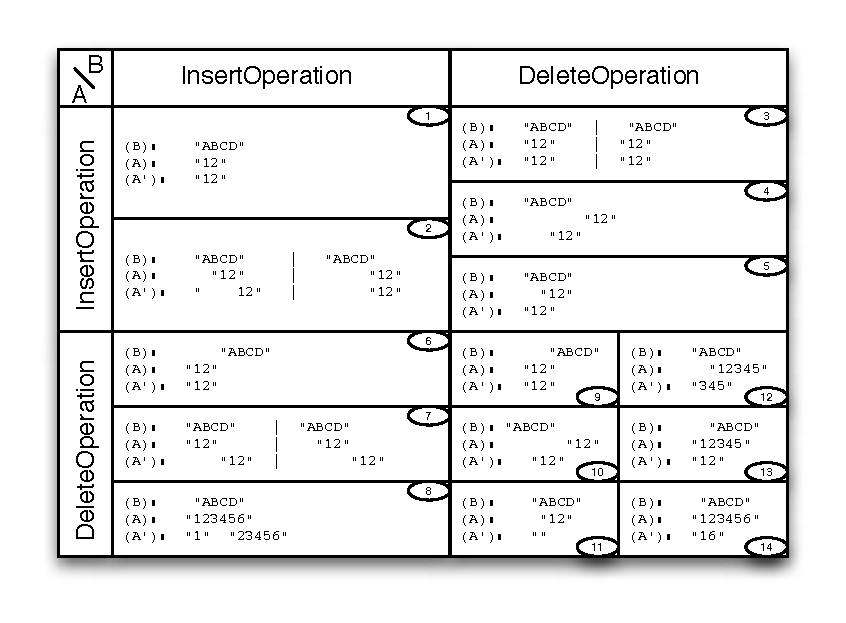
\includegraphics[height=12cm,width=16cm]{../../images/algo-impl/transform_overview.eps}
\caption{Transformation Overview}
\label{Transformation Overview}
\end{figure}

\subsubsection{Insert/Insert}
- some position problem
  - char
    - counter example
  - origin
    - problem
  - isTransformOpPrivileged
\begin{itemize}
\item \textbf{Case 1:}
Operation A starts before operation B. Nothing has to be transformed.
\item \textbf{Case 2:}
Operation A starts in or behind operation B. Index of operation A' must be increased by the length of the text of operation B.
\end{itemize}

\subsubsection{Insert/Delete}
\begin{itemize}
\item \textbf{Case 3:}
Operation A starts before or at the same position as operation B. Nothing has to be transformed.
\item \textbf{Case 4:}
Operation A starts after operation B. Index of operation A' must be reduced by the length of the text of operation B.
\item \textbf{Case 5:}
Operation A starts in operation B. Index of A' must be the index of operation B.
\end{itemize}

\subsubsection{Delete/Insert}
\label{Delete_Insert}
- splitoperation
\begin{itemize}
\item \textbf{Case 6:}
Operation A is completly before operation B. Nothing has to be transformed.
\item \textbf{Case 7:}
Operation A starts before or at the same position as operation B. Index of operation A' must be increased by the length of the text of operation B.
\item \textbf{Case 8:}
Operation B is in the range of operation A. Operation A' must be splitted up into two delete operations. For more details about this process see \cite{Delete_Insert}.
\end{itemize}

\subsubsection{Delete/Delete}
\begin{itemize}
\item \textbf{Case 9:}
Operation A is completly before operation B. Nothing has to be transformed.
\item \textbf{Case 10:}
Operation A starts at the end or after operation B. Index of operation A' must be reduced by the length of the text of operation B.
\item \textbf{Case 11:}
Operation A and operation B are overlapping. Operation B starts before or at the same position as operation A and ends after or at the same position as operation A. Content of operation A has been allready deleted by operation B. Nothing has to be deleted by operation A. A' is called a noop (no-operation).
\item \textbf{Case 12:}
Operation A and operation B are overlapping. Operation B starts before or at the same position as operation A and ends before operation A. The overlapping part of the two operations has been deleted by operation B. Operation A' has to delete only the remaining text (text after the overlapping text of the two operations).
\item \textbf{Case 13:}
Operation A and operation B are overlapping. Operation B starts after operation A and ends after or at the same position as operation A. The overlapping part of the two operations has been deleted by operation B. Operation A' has to delete the remaining text (text before the overlapping text of the two operations).
\item \textbf{Case 14:}
Operation A and operation B are overlapping. Operation B is fully in operation A. The overlapping part of the two operations has been deleted by operation B. Operation A' has to delete the remaining text (text before and after the overlapping text of the two operations).
\end{itemize}



\subsection{Client}


\subsection{Server}


\subsection{Undo/Redo}


\subsection{Tests}

